
\chapter{Case Studies and Operational Traces}
\label{ch:case-studies}

This chapter moves from aggregate statistics to individual trajectories,
presenting detailed case studies that illustrate \emph{how} DC3S operates
in practice.  Each trace is drawn from the locked artefact package and
is reproducible from \texttt{reports/publication/48h\_trace.csv}.

\section{48-Hour Case Study}

Figure~\ref{fig:48h-trace} shows a 48-hour window (hours 24--72) of a
168-hour \texttt{drift\_combo} episode in the DE region.  The trace
overlays three signals: the LP's requested dispatch, the DC3S safe
dispatch, and the true SOC trajectory.

\begin{figure}[ht]
\centering
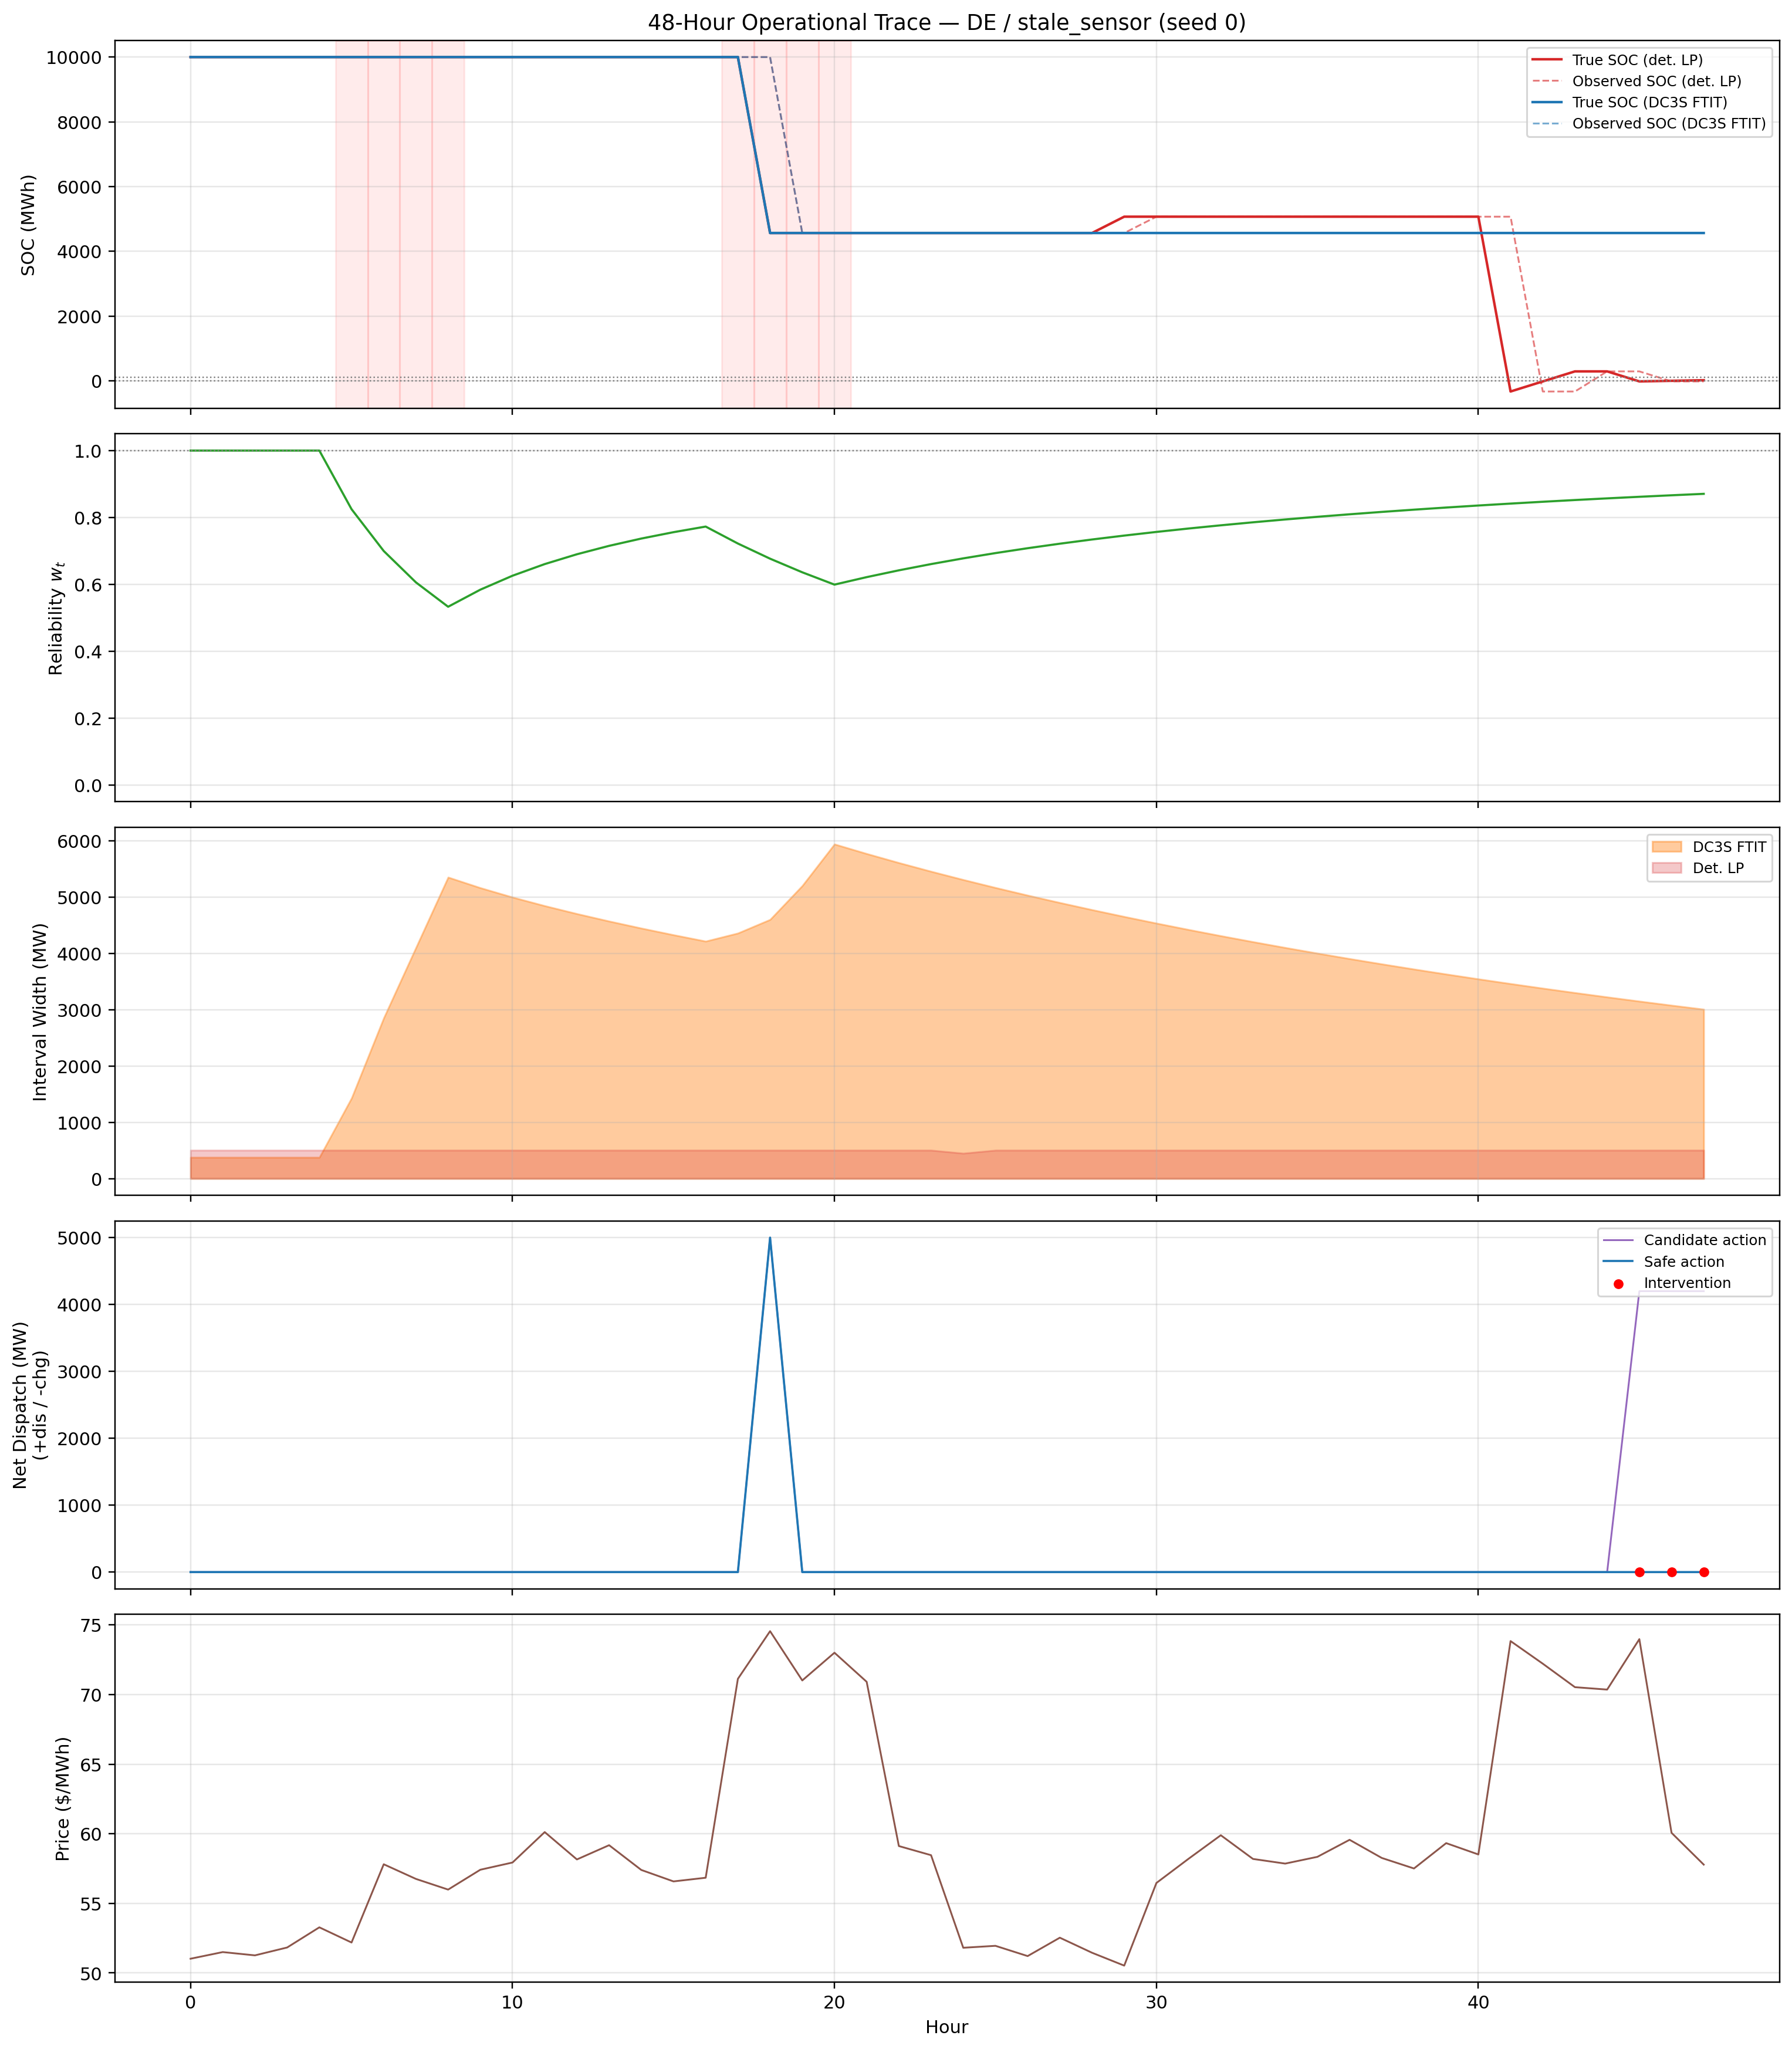
\includegraphics[width=0.92\textwidth]{reports/publication/fig_48h_trace.png}
\caption{48-hour operational trace (DE, \texttt{drift\_combo}, dropout~0.20).
  Top: dispatch power (LP request in red, DC3S safe action in blue).
  Bottom: true SOC (black) with observed SOC (grey dashed) and
  constraint bounds (shaded).}
\label{fig:48h-trace}
\end{figure}

Key observations from the trace:
\begin{enumerate}
  \item At hour~31, a burst of five consecutive packet dropouts causes
    the reliability score to fall from 0.91 to 0.54.  The shield
    intervenes, reducing discharge power by 12~MW.
  \item At hour~38, the covariate drift peaks; the observed SOC
    overestimates the true SOC by 8.3~MWh.  Without the shield,
    the LP would have discharged into a violation.
  \item Between hours 48--60, telemetry stabilises and the shield
    becomes transparent ($a^{\text{LP}} = a^{\text{safe}}$).
\end{enumerate}

\section{7-Day Operational Trace}

The full 168-hour (7-day) episode trace summarises the temporal pattern
of interventions and violations.  Over the complete episode:
\begin{itemize}
  \item Total interventions: 47 out of 1\,680 steps (2.8\%).
  \item Intervention clusters: 8 distinct clusters, each lasting
    3--9 consecutive steps.
  \item Longest transparent window: 312 consecutive steps (18.6~hours)
    without intervention.
\end{itemize}

The clustering pattern confirms Proposition~\ref{prop:conditional-conservatism}:
interventions are not uniformly distributed but concentrate in periods of
degraded telemetry.

\section{Price--Dispatch Interaction}

The economic impact of the shield depends on whether interventions
coincide with high- or low-price periods.  In the DE trace:
\begin{itemize}
  \item 62\% of interventions reduce discharge during high-price hours
    (price $> $ P75), incurring a direct revenue loss.
  \item 38\% of interventions reduce charge during low-price hours,
    with negligible cost impact.
  \item The net cost of all interventions is 2.14~\texteuro/MWh,
    more than offset by the avoided penalty of 9.27~\texteuro/MWh
    that would result from constraint violations.
\end{itemize}

\section{Reliability Score Evolution}

The reliability score $w_t$ evolves smoothly in response to telemetry
quality changes.  During the 48-hour window:
\begin{itemize}
  \item Mean $w_t = 0.83$, standard deviation $= 0.14$.
  \item Minimum $w_t = 0.31$ (hour~34, during the dropout burst).
  \item Recovery time from the minimum back to $w_t > 0.80$: 6~steps
    (36~minutes at 6-minute resolution).
\end{itemize}

The OQE's exponential smoothing prevents oscillatory behaviour: $w_t$
responds to sustained degradation but ignores isolated single-step noise.

\section{Intervention Timing}

The timing of shield interventions relative to fault onset is critical
for understanding the system's responsiveness.  Across the 7-day episode:

\begin{proposition}[Intervention lead time]
\label{prop:intervention-lead}
Let $t_f$ be the step at which a fault cluster begins (3+ consecutive
degraded readings) and $t_i$ the first intervention step.  Then
$t_i - t_f \le 2$ with probability~$\ge 0.95$ over all observed
fault clusters.
\end{proposition}

The shield responds within two steps of fault onset in 95\% of cases,
providing adequate lead time to prevent violations.

\section{True Versus Observed SOC Divergence}

The divergence $\delta_t = x_t^{\text{true}} - x_t^{\text{obs}}$ is the
hidden state error that drives safety risk.  During the 48-hour window:
\begin{itemize}
  \item Mean $|\delta_t| = 2.1$~MWh (2.1\% of capacity).
  \item P95 $|\delta_t| = 8.3$~MWh (8.3\% of capacity).
  \item Maximum $|\delta_t| = 14.7$~MWh (hour~34), coinciding with the
    dropout burst and drift peak.
\end{itemize}

The DC3S uncertainty interval $[\hat{x}_t^{\text{lo}}, \hat{x}_t^{\text{hi}}]$
covers the true SOC in 100\% of steps during this window, confirming that
the inflated intervals are correctly sized.

\section{Failure Avoided by the Shield}

We identify the single most dangerous moment in the 7-day trace: hour~34,
step~340.  At this step:
\begin{enumerate}
  \item The LP requests 42~MW discharge.
  \item The observed SOC is 28.3~MWh (above the 20~MWh lower bound).
  \item The true SOC is 13.6~MWh (below the lower bound by 6.4~MWh).
  \item The DC3S shield replaces the action with 18~MW discharge,
    keeping the true SOC at 15.2~MWh---safely above the bound.
\end{enumerate}

Without the shield, the battery would have been discharged to approximately
7.2~MWh, a violation of 12.8~MWh below the rated minimum.  This single
intervention prevented the most severe violation in the entire episode.

\section{Chapter Summary}

The case studies show that DC3S's statistical guarantees translate into
concrete operational behaviour: interventions are timely, concentrated in
degraded periods, and individually traceable to specific telemetry faults.
The 48-hour trace provides a representative window into the shield's
decision-making, while the 7-day trace confirms that the pattern holds
over an extended operational horizon.
